%\newpage

\section{Balancing coarse-grained parallelism and locality}
\label{selection}

There are many loop transformation techniques that exists today\cite{All02}. And almost all of them can be applied to more than
one kind of code optimizations. For example, loop interchange is
widely used to improve data locality in cache management. Meanwhile, it
also can be used to exploit parallelism, such as vectorization, and
even coarse-grained parallelism.  Unfortunately, the transformations
for different optimization purposes do not always work in harmony.

For instance, in a loop nest, maximum spatial cache reuse can be achieved by moving the loop with stride-one access of the references to the innermost position. So a loop permutation
algorithm will try to calculate such a loop order while keeping the
dependence constraints of the original loop nest. On the other hand, in an automatic parallelizing compiler, one would
like to parallelize the outermost loop to reduce the parallel region
setup overhead, and leave more code in the inner loop for other
optimization opportunities. 

There has been significant research to study different approaches to solve this problem.
A well known technique is \emph{Unimodular transformation}
\cite{Mic91,Lam91,Ban90}, a compound loop transformation algorithm aiming at
integrating different loop transformations for a specific goal and
target machine, thereby reducing the problem of finding the best
transformation combination to finding the best unimodular matrix. Another technique is \emph{Loop selection}\cite{All02}, which
parallelizes all the parallelizable loops, then uses heuristics to
select the next one as sequential, expecting to find more
parallelizable loops after that. This is easier to implement when compared to
unimodular transformation.

Our work is based on the idea of loop selection, but is different from
the original one in two aspects: a) given our target is an OpenMP node
program, we only need to find one parallelizable loop per nest, to avoid
generating code with nested parallelism; b) our heuristics are
directly linked to data locality, unlike the original loop selection
technique which picks a loop with most ``$<$'' directions to parallelize.

\subsection{Analyzing model}

Using the notation in Section \ref{par_structure}, we introduce two
theorems.

\begin{theorem}[C-level interchangeable] \label{theorem:interchange}
  Loop $L_{c}$ and $L_{c-1}$ is interchangeable if and only if   
   $\forall \vec{\delta} \in \mathcal{D}$, $\vec{\delta} \neq
  (=^{(c-2)} < > \ldots)$, where ``$=^{(c-2)}$'' indicates that there are
  $(c-2)$ directions as ``$=$'' before the first ``$<$''.
\end{theorem} 

Theorem \ref{theorem:interchange} and its variant forms can be found
in \cite{Zim90} and other literatures. We will not prove it here, but 
use it directly for our theorem later.

\begin{theorem}[P-level parallelizable] \label{theorem:parallelize}
  Loop $L_{p}$ can be parallelized as a parallel do if and only if
   $\forall \vec{\delta} \in \mathcal{D}$, $\vec{\delta} \neq
  (=^{(p-1)} < \ldots)$.
%, where ``$=^{(p-1)}$'' means there are $(p-1)$
%  directions as ``$=$'' before the first ``$<$''.
\end{theorem} 

The proof for Theorem \ref{theorem:parallelize} is trivial. By the
definition of parallel do, it cannot carry any dependence.

Next, we define a \emph{multiply} operation on a dependence vector.
Let $ \vec\sigma=\vec{\sigma}_{a} \times \vec{\sigma}_{b}$, where
$\forall \sigma_{j} \in \vec\sigma, \sigma_{j} = \sigma_{a_{j}} \times
\sigma_{b_{j}}$. The multiplication of the two dependence distances is
defined as following. It is unknown if one of the distances is unknown.
Otherwise, it will be the regular multiplication on two integers. If
one of the distances is only a direction, it is treated as 1 or -1, and
after the multiplication, converted back to a direction .

Let $\vec{\sigma}_{p}$ and $\vec{\sigma}_{p-1}$ be the $p^{th}$,
$(p-1)^{th}$ column vector of dependence matrix $\mathcal{D}$, then we
have

\begin{theorem}[Keeping it parallelizable] \label{theorem:keep}
  A p-level parallelizable loop $L_{p}$ can be interchanged to
  $L_{p-1}$ and becomes (p-1)-level parallelizable if and only if 
  $\forall \sigma_{j} \in \vec{\sigma}$, where $\vec{\sigma} =
  \vec{\sigma}_{p-1} \times \vec{\sigma}_{p}$, either
  \begin{itemize}
  \item $\sigma_{j}=0$ or 
  \item the $j^{th}$ dependence in $\mathcal{D}$ is not carried by
    $L_{p-1}$
  \end{itemize}
\end{theorem} 

\begin{flushleft}
\textbf{Proof} 
\end{flushleft}

We start by proving the ``\emph{if}'' part of the theorem.

Suppose $\forall \sigma_{j}=0$. 

First, we can assert that $L_{p-1}$ and
$L_{p}$ is interchangeable. Otherwise, according to Theorem
\ref{theorem:interchange} there is a dependence vector $\vec{\delta}$
that has the form of $(=^{(p-2)} < > \ldots)$. This will conflict with the
fact that all $\sigma_{j}$ is zero.
Secondly, we prove that the $L_{p}$ will become $(p-1)$-level
parallelizable after interchanging with $L_{p-1}$.  Otherwise, from
Theorem \ref{theorem:parallelize}, there will a dependence vector
$\vec{\delta}$, of the format $(=^{(p-2)} < \ldots)$, in the
dependence matrix preventing it from being parallelized after the
interchange. Considering the format of the $\vec{\delta}$ before the
interchange, given that all $\sigma_{j}$ is zero, it should be in the
form of $(=^{(p-1)} < \ldots)$. This conflicts with the fact that $L_{p}$
is parallelizable according to Theorem \ref{theorem:parallelize}.

If $\exists \sigma_{j} \neq 0$, we let $\vec{\delta}$ be the
dependence vector on the $j^{th}$ row of the matrix. It should have
one of the following formats $(\cdots^{(p-2)} < < \ldots)$,
$(\cdots^{(p-2)} < > \ldots)$, $(\cdots^{(p-2)} > < \ldots)$,
$(\cdots^{(p-2)} > > \ldots)$, where $\cdots^{(p-2)}$ is the leading
$(p-2)$ positions. Since $L_{p-1}$ does not carry any dependences as
in the given condition, $\cdots^{(p-2)}$ has to be in the format of
$(= \ldots = < \ldots)$, in order for the $\delta$ to be valid. Therefore,
$L_{p}$ can be interchanged with $L_{p-1}$ and still be kept parallelizable.

Similarly, the ``\emph{only if}'' part of the theorem can be proved. This is not important in our algorithm, so we will omit it here.

\begin{flushright}
\textbf{End of Proof} 
\end{flushright}

\begin{theorem}[Outermost parallelizable] \label{theorem:outermost}
  Loop $L_{o}$ can be parallelized at the outermost level if and only
  if  $\vec{\sigma} = \vec{0}$, where $\vec{\sigma}$ is the
  $o^{th}$ column vector of dependence matrix $\mathcal{D}$.
\end{theorem} 

This is a direct conclusion from Theorem \ref{theorem:keep}. It is
actually used in \cite{All02} for loop selection.

\subsection{Loop permutation with examples}
\label{sec:algorithms}


%{\small
%\begin{algorithm}[h]
%%  \SetLine %this is for setting vertical line with keyword end
%  \SetKw{KwBreak}{break}
%  \SetKwInOut{Input}{Input}
%  \SetKwInOut{Output}{Output}
%  \Input{A desired loop permutation order $O=(L_1,L_2,...,L_n)$, \\
%    the original dependence matrix $\mathcal{D}$ for the loop}
%  \Output{A nearby permutation $P$}
%  \BlankLine

%  \Begin {
%    \If{$\forall \delta \in \mathcal{D}$, $O$ is legal}{
%      \KwRet $O$ \;
%    }
%    $P:=\emptyset$; $k:=0$; $m:=n$\;
%    \While{$O \neq \emptyset$} {
%      \For{$i:=1$ \KwTo $m$} {
%        \If {$\forall \delta, (P_1,...,P_k, L_i)$ is legal} {
%          $P:=(P_1,...,P_k, L_i)$ \;
%          $O:=O-\{L_i\}$\; 
%          $k:=k+1$; $m:=m-1$ \;
%          \KwBreak
%        }
%%        select the leftmost loop $l$ in $O$ \\
%%        such that $(P_1,P_2,...,P_{i-1},l)$ has no illegal direction vector prefixes \;
%%        remove $l$ from $O$ \;
%%        append $l$ to the end of $P$, so that it becomes $P_i$ \;
%      }
%    }
%  }
%  \caption{Select a permutation for data locality}
%  \label{alg:permutelocal}
%\end{algorithm}
%}

Based on our discussion in the previous section, we try to find a
permutation favoring both data locality and parallelism. To do this, 
we first assign each loop induction variable with a weight in terms
of memory access. We will favor those having maximum memory spatial
reuse.  A more comprehensive way of evaluating the weights is called
profitability-based methods, introduced in \cite{All02}, which has a
cache model to estimate cache misses. Either way, a memory ordering
$O=(L_1,L_2,...,L_n)$ of the nested loops is calculated, where $L_1$
has the least reuse and $L_n$ the most.

Next we build up a nearby legal permutation in $P$ by first testing to see if the loop $L_1$ is
legal in the outermost position.  If it is legal, it is added to $P$
and removed from $O$. If it is not legal, the next loop in $O$ is
tested.  Once a loop $L_{i}$ is positioned, the process is repeated
starting from the beginning of $O-\{L_{i}\}$ until $O$ is empty. $P$
is considered as having the best data locality for the loop nest. The algorithm is summarized in \cite{Mck96},

%{\small
%\begin{algorithm}[h]
%%  \dontprintsemicolon
%%  \SetLine %this is for setting vertical line with keyword end
%  \SetKw{KwBreak}{break} 
%  \SetKwInOut{Input}{Input}
%  \SetKwInOut{Output}{Output}
%  \Input{A loop order $O=(L_1,L_2,...,L_n)$ in favor of data locality, \\
%    the original dependence matrix $\mathcal{D}$ for the loop}
%  \Output{A permutation $P$ considering coarse-grained parallelism as
%    well} 
%  \AlgData{two integers $src$, $dst$ to represent preferred move}

%  \BlankLine

%  \Begin {
%    \If{$L_1$ is parallelizable} {
%      \KwRet $O$ \;
%    }
%    $src:=n$; $dst:=n$ \;
%    \For {$i:=2$ \KwTo $n$} {
%      \If {$L_i$ is parallelizable} {
%        \For {$j:=i-1$ \KwTo $1$} {
%          \If {$L_i$ can be moved before $L_j$} {
%            \If {$j < dst$} {
%               $src:=i$; $dst:=j$ \;
%               \lIf{$dst=1$} {\KwBreak}
%            }
%          }
%        }
%        \lIf{$dst=1$} {\KwBreak}
%      }
%    }
%    construct $P$ with $src$ and $dst$ 
%  }
%  \caption{Select a permutation for parallelism}
%  \label{alg:permutepar}
%\end{algorithm}
%}

%Finally, we use Algorithm \ref{alg:permutepar} to do further
%adjustment. Given all the parallelizable loops in the nest, it try to
%move a parallelizable loop outer as much as possible.

Finally, we can adjust the other loops further, based on the
following conditions to decide if $L_i$ can be moved before $L_j$,

\begin{itemize}
\item The interchange should be legal,
\item $L_i$ is still parallelizable after moving, and
\item The amount of data locality we are willing to sacrifice.
\end{itemize}

The first two questions are answered by Theorem \ref{theorem:keep}.
We will use heuristics including the induction variable weights
calculated previously to control how aggressive the parallelizer
should be. Apart from estimating the cache miss, a good heuristic could
also include estimations of the loop cost and parallel setup overhead. The
topics deserve some discussions on their own, and will not be
included here. \emph{Strip-mining} can also be considered, if no
loop can be moved at all.

%We used an XL FORTRAN 8.1 based development compiler on an 8 node
%1.1GHz POWER4 system to do the following test. 

We illustrate the benefits of using our loop permutation algorithm using a simple example. Loop permutation for data locality will transform the Fortran code shown below to \texttt{K} loop as the outermost and \texttt{I} loop as the innermost in the nest. This
will lead to the middle \texttt{J} loop getting parallelized. With our loop
permutation algorithm we can have the \texttt{J} loop moved to the
outermost position, thus striking a balance between locality and the desired coarse-grained parallelism.

{\small
\begin{verbatim}
 DO I = 1, N
   DO J = 1, N
     DO K = 1, N 
       A(I,J,K)=A(I,J,K+1);
     END DO
   END DO
 END DO
\end{verbatim}
}


%{\small
%\begin{verbatim}
% DO K = 1, N
%   DO J = 1, N
%     DO I = 1, N 
%       A(I,J,K)=A(I,J,K+1);
%     END DO
%   END DO
% END DO
%\end{verbatim}
%}

%Since \texttt{I} has stride-one access to the array \texttt{A}, it
%will be moved to the innermost position. If we enable the
%auto-parallelizer, compiler will generate code roughly corresponding
%the following segment,

%{\small
%\begin{verbatim}
%      DO K = 1, N
%!OMP$ PARALLEL DO
%        DO J = 1, N
%          DO I = 1, N
%            A(I,J,K)=A(I,J,K+1);
%          END DO
%        END DO
%      END DO
%\end{verbatim}
%%$ closing dolar
%}

%With Algorithm \ref{alg:permutepar} implemented, the final results can
%be further improved as,

%{\small
%\begin{verbatim}
%!OMP$ PARALLEL DO
%      DO J = 1, N
%        DO K = 1, N
%          DO I = 1, N 
%            A(I,J,K)=A(I,J,K+1);
%          END DO
%        END DO
%      END DO
%\end{verbatim}
%%$ closing dolar
%}

\begin{figure}[!t]
  \begin{center}
    % run boxfill.pl to get the filled version of the graph
    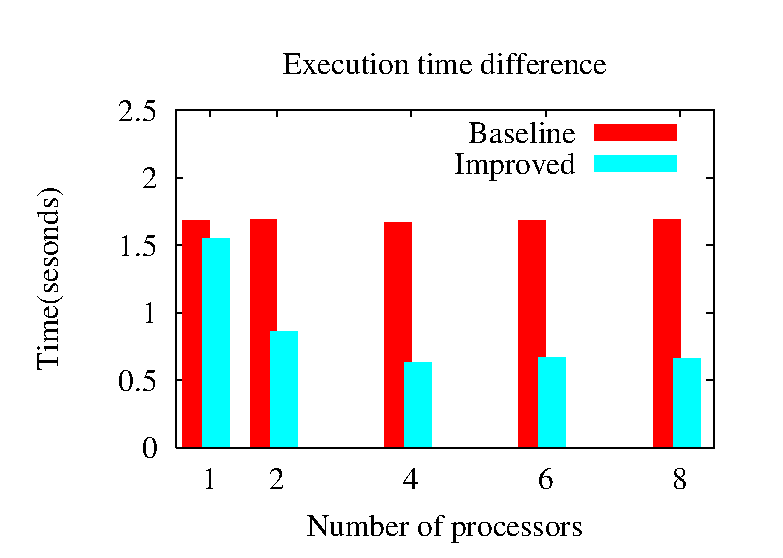
\includegraphics[angle=0, width=0.55\textwidth]{compare.eps}
    \caption{\footnotesize Performance difference}
    \label{fig:compare}
  \end{center}
\end{figure}

Figure \ref{fig:compare} shows the performance difference of the
generated code on the POWER4 system for both the cases discussed. \texttt{N} is set to 100 and the loop nest is executed 100 times. In the figure, ``Baseline'' and
``Improved'' use exactly the same compiler, with the only difference being that the parallel loop
is in the middle for the ``Baseline'' case and the outermost for the ``Improved'' case. We can see that the parallel setup overhead completely offsets the gain from parallelization in the first case,
while the improved version sees reasonable speedup even for a loop with 
small computation cost (the loop body has a single assignment statement).

In the SPEC2000FP suite, \texttt{mgrid} was negatively affected by this
transformation, further experiments are being carried out to derive better heuristics.
